%\documentclass[12pt]{article}

\questionheader{ex:s1.6}

%%%%%%%%%%%%%%%%%%
\subsection*{\Conceptual}
%%%%%%%%%%%%%%%%%%
%%%%%%%%%%%%%%%%%%%
%%%%%%%%%%%%%%%
%%%%%%%%%%%%%%%%%%%
\begin{question}
Give an equation for arclength of a curve $C$ as a line integral.
\end{question}
\begin{hint}
Your differential is $\dee{s}$, where $s$ is arclength.
\end{hint}
\begin{answer}
$\int_C \dee{s}$
\end{answer}
\begin{solution}
We want to add up all the tiny pieces of arclength $\dee{s}$ along a curve $C$. So, the integral would simply be $\int_C \dee{s}$.

To see this another way, if we define $\vr=(x(t),y(t),z(t))$ for $a \le t \le b$ to be the equation of $C$, we could calculate the arclength as:
\begin{align*}
\int_a^b |\vr'(t)|\dee{t}&=\int_a^b \sqrt{x'(t)^2+y'(t)^2+z'(t)^2}\dee{t}
\end{align*}
This fits the form of Definition~\eref{CLP317}{def:lineIntegral} with $f(x,y,z)=1$, so we write it as a line integral as $\int_C 1 \dee{s}$, which is equivalent to $\int_C \dee{s}$.
\end{solution}


%%%%%%%%%%%%%%%%%%%
\begin{question}
\begin{enumerate}[(a)]
\item
Show that the integral $\int_\cC f(x,y)\,ds$ 
along the curve $\cC$ given in polar coordinates by 
$r=r(\theta)$, $\theta_1\le \theta\le\theta_2$, is
\begin{equation*}
\int_{\theta_1}^{\theta_2}f\big(r(\theta)\cos\theta, r(\theta)\sin\theta\big) \sqrt{r(\theta)^2+\left(\diff{r}{\theta}(\theta)\right)^2}\,
\dee{\theta}
\end{equation*}

\item
Compute the arc length of $r=1+\cos\theta,\ 0\le \theta\le 2\pi$.
You may use the formula
\begin{equation*}
1+\cos\theta=2\cos^2\frac{\theta}{2}
\end{equation*}
to simplify the computation.	
\end{enumerate}
\end{question}

\begin{hint}
(a) You can parametrize the curve by 
   $\vr(\theta) = r(\theta)\,\cos\theta\,\hi +
                  r(\theta)\,\sin\theta\,\hj$, $\theta_1\le \theta\le\theta_2$.
\end{hint}

\begin{answer}
(a) See the solution.\qquad
(b) $8$
\end{answer}

\begin{solution}
(a) The curve is 
$\vr(\theta) = x(\theta)\,\hi+ y(\theta)\,\hj$
with $x(\theta)=r(\theta)\cos\theta$, $y(\theta)=r(\theta)\sin\theta$ 
and $\theta_1\le \theta\le \theta_2$.
On this curve 
\begin{align*}
\vv(\theta) =\diff{\vr}{\theta}(\theta)&= x'(\theta)\hi+ y'(\theta)\hj
=\big[r'(\theta)\cos\theta-r(\theta)\sin\theta\big]\hi+
\big[r'(\theta)\sin\theta+r(\theta)\cos\theta\big]\hj\cr
\implies  \diff{s}{\theta}(\theta)
&=\sqrt{\big[r'(\theta)\cos\theta-r(\theta)\sin\theta\big]^2
+ \big[r'(\theta)\sin\theta+r(\theta)\cos\theta\big]^2}\cr
&=\sqrt{r'(\theta)^2+r(\theta)^2}
\end{align*}
Hence
\begin{align*}
\int_\cC f(x,y)\,ds 
&= \int_{\theta_1}^{\theta_2}\!\!\!f\big(x(\theta), y(\theta)\big) \diff{s}{\theta}\,\dee{\theta}
\cr
&=\int_{\theta_1}^{\theta_2}\!\!\!f\big(r(\theta)\cos\theta, r(\theta)\sin\theta\big) \sqrt{r(\theta)^2
     +\left(\diff{r}{\theta}(\theta)\right)^2}\,
\dee{\theta}
\end{align*}

(b)
In this case $f(x,y)=1$, $r(\theta)=1+\cos\theta$, $\theta_1=0$ and $\theta_2=2\pi$,
\begin{align*}
\int_C \,ds
&=\int_0^{2\pi} \sqrt{[1+\cos\theta]^2+[-\sin\theta]^2}\,\dee{\theta}
=\int_0^{2\pi} \sqrt{2(1+\cos\theta)}\,\dee{\theta}\cr
&=\int_0^{2\pi} \sqrt{4\cos^2\frac{\theta}{2}}\,\dee{\theta}
=2\int_0^{2\pi} \left|\cos\frac{\theta}{2}\right|\,\dee{\theta}
=4\int_0^{\pi} \cos\frac{\theta}{2}\ \dee{\theta}
=8 \sin\frac{\theta}{2}\bigg|_0^{\pi}
=8
\end{align*}
\end{solution}

%%%%%%%%%%%%%%%%%%%
%\begin{question}
%Evaluate $\int_\cC x^2y^2\,\dee{x}$ along the line segment from 
%$(0,1)$ to $(1,1)$. (When we move to the right from $(x,1)$ to $(x+\dee{x},1)$
%with $\dee{x}>0$, the distance moved is $\dee{s}=\dee{x}$. So in this case, 
%it is common to write
%$\int_\cC x^2y^2\,\dee{x}$ in place of $\int_\cC x^2y^2\,\dee{s}$.)
%\end{question}
%
%\begin{hint}
%The line segement $\cC$ can be easily parameterized using $x$
%as the parameter. 
%\end{hint}
%\begin{answer}
%$\frac{1}{3}$
%\end{answer}
%\begin{solution}
%We may parametrize $\cC$ by $\vr(x)=x\,\hi+\hj$ with $0\le x\le 1$.
%So $\big|\diff{\vr}{x}(x)\big| = |\hi|=1$ and 
%\begin{align*}
%\int_\cC x^2y^2\,\dee{x}
%&=\int_0^1 x^2 \overbrace{(1)^2}^{y^2}\ \left|\diff{\vr}{x}(x)\right|\,\dee{x} \\
%&=\int_0^1 x^2 \,\dee{x} \\
%&=\frac{1}{3}
%\end{align*}
%
%\end{solution}


%%%%%%%%%%%%%%%%%%%
%%%%%%%%%%%%%%%%%%%


%%%%%%%%%%%%%%%%%%%

%%%%%%%%%%%%%%%%%%
\subsection*{\Procedural}

%%%%%%%%%%%%%%%%%%%%%%%%%
\begin{question}
Calculate $\int_C \left(\frac{xy}{z}\right)\dee{s}$, where $C$ is the curve $\left( \frac23t^3~,~\sqrt{3}t^2~,~3t \right)$ from $t=1$ to $t=2$.
\end{question}
\begin{hint}
Following Definition~\eref{CLP317}{def:lineIntegral}, set $f(x,y,z)=\frac{xy}{z}$, $x(t)=\frac23 t^3$, $y(t)=\sqrt3t^2$, and $z(t)=3t$.
\end{hint}
\begin{answer}
$ \frac{4}{21\sqrt 3}(2^7-1) + \frac{2}{5\sqrt 3}(2^5-1)$
\end{answer}
\begin{solution}
Following Definition~\eref{CLP317}{def:lineIntegral}:
\begin{align*}
\int_C \left(\frac{xy}{z}\right)\dee{s}&=\int_1^2 \left(\frac{\frac23t^3 \cdot \sqrt{3}t^2}{ 3t} \right)\sqrt{(2t^2)^2+(2\sqrt3 t)^2+(3)^2}\,\dee{t}\\
&=\int_1^2 \left(\frac{2}{ 3\sqrt 3} \,t^4\right)(2t^2+3)\,\dee{t} = \frac{4}{21\sqrt 3}(2^7-1) + \frac{2}{5\sqrt 3}(2^5-1)
\end{align*}
\end{solution}
%%%%%%%%%%%%%%%%%%%%%%%%%%%%%%%
%%%%%%%%%%%%%%%%%%%
\begin{question}
	A hoop of radius $1$ traces out the curve $x^2+y^2=1$, where $x$ and $y$ are measured in metres. At a point $(x,y)$, its density is $x^2$ kg per metre. What is the mass of the hoop?
\end{question}
\begin{hint}
	Parametrize the circle in the usual way.
\end{hint}
\begin{answer}
	$\pi$ kg
\end{answer}
\begin{solution}
	We parametrize the unit circle as $(\cos t, \sin t)$, $0 \le t \le 2\pi$.
	
		A tiny slice of the hoop with length $\dee{s}$ has mass $(x^2~ \mathrm{kg}/\mathrm{m})(\dee{s}~ \mathrm{m})=x^2\dee{s}~ \mathrm{kg}$. So, the entire hoop has mass:
		\begin{align*}
			\int_C x^2\,\dee{s}&=\int_0^{2\pi} \cos^2 t \sqrt{(-\sin t)^2+(\cos t)^2}\,\dee{t}=\int_0^{2\pi} \cos^2 t \,\dee{t}\\
&=\int_0^{2\pi} \frac{1+\cos(2t)}{2}\ \dee{t}
                 =\left[\frac{t}{2} +\frac{\sin(2t)}{4} \right]_0^{2\pi}=\pi ~\mathrm{kg}
			\end{align*}
			 For an efficient, sneaky, way to evaluate 
                 $\int_0^{2\pi} \cos^2 t\ \dee{t}$, see Example
                 \eref{CLP317}{eg:workIntegalB} in the CLP-4 text.
\end{solution}

%%%%%%%%%%%%%%%%%%%
\begin{question}
	Compute $\int_C (xy+z) \dee{s}$ where $C$ is the straight line from $(1,2,3)$ to $(2,4,5)$.
\end{question}
\begin{hint}
	$C$ can be parametrized as $(1+t,2+2t,3+2t)$ for $0 \le t \le 1$.
\end{hint}
\begin{answer}
	$26$
\end{answer}
\begin{solution}
	To parametrize $C$, we note the vector between the two points is $(2-1,4-2,5-3)=(1,2,2)$. So, the line is $(1,2,3)+t(1,2,2)$ for $0 \le t \le 1$. That is, $x(t)=1+t$, $y(t)=2+2t$, and $z(t)=3+2t$.
	\begin{align*}
		\int_C(xy+z)\dee{s}&=\int_0^1 \left((1+t)(2+2t)+(3+2t)\right)\sqrt{1^1+2^2+2^2}\dee{t}\\
		&=              \int_0^1 3\big(5 + 6t + 2t^2\big)\ \dee{t}=26
		\end{align*}
\end{solution}


%%%%%%%%%%%%%%%%%%%
\begin{question}
Evaluate the path integral $\int_\cC f(x,y,z)\,\dee{s}$ for
\begin{enumerate}[(a)]
\item 
$f(x,y,z)=x\cos z$, \ \ \ $\cC:\vr(t)=t\hi+t^2\hj$,
$0\le t\le 1$.

\item $f(x,y,z)=\frac{x+y}{y+z}$, \ \ \ \ \ \ 
$\cC:\vr(t)= \big(t,\frac{2}{3}t^{3/2},t\big)$,
$1\le t\le 2$.	
\end{enumerate}
\end{question}

%\begin{hint}
%\end{hint}

\begin{answer}
(a) $\frac{5^{3/2}-1}{12}$\qquad
(b) $\frac{8-3^{3/2}}{3/2}$	
\end{answer}

\begin{solution}
(a) 
In this case $\vr(t)=t\hi+t^2\hj$, so that
$\vv(t)=\diff{\vr}{t}(t)=\hi+2t\hj$ and $\diff{s}{t}=\sqrt{1+4t^2} $. Hence
\begin{align*}
\int_\cC f(x,y,z)\,\dee{s}
&=\int_0^1 x(t)\cos z(t) \diff{s}{t}\,\dee{t}
=\int_0^1 t(\cos 0) \sqrt{1+4t^2}\,\dee{t}
=\frac{1}{8}\frac{ {(1+4t^2)}^{3/2}}{3/2}\bigg|_0^1\\
&=\frac{5^{3/2}-1}{12}
\end{align*}

(b) In this case $\vr(t)=\big(t,\frac{2}{3}t^{3/2},t\big)$, so
that
$\vv(t)=\diff{\vr}{t}(t)=\big(1,t^{1/2},1\big)$ and 
$\diff{s}{t}=\sqrt{2+t} $. Hence
\begin{align*}
\int_\cC f(x,y,z)\,\dee{s}
&=\int_1^2 \frac{x(t)+y(t)}{y(t)+z(t)} \, \diff{s}{t}\,\dee{t}
=\int_1^2 \frac{t+{2\over 3}t^{3/2}}{{2\over3}t^{3/2}+t} \sqrt{2+t}\,\dee{t}
=\frac{(2+t)^{3/2}}{3/2}\bigg|_1^2 \\
&=\frac{8-3^{3/2}}{3/2}
\end{align*}	

\end{solution}



%%%%%%%%%%%%%%%%%%%%%%%%%
\begin{question}
	Evaluate $\int_C \sin x\,\dee{s}$, where $C$ is the curve $(\arcsec(t), \ln t)$, $1 \le t \le \sqrt{2}$. 
\end{question}
\begin{hint}
	Simplify! Also: $\diff{}{t}\{\arcsec t\} = \frac{1}{|t|\sqrt{t^2-1}}$.
\end{hint}
\begin{answer}
	$\frac12 \ln 2$
\end{answer}
\begin{solution}
  In the figure below, we construct a triangle with $\theta=\arcsec t$; the hypotenuse has length $t$, while the side adjacent to $\theta$ has length 1. By the Pythagorean Theorem, the remaining side has length $\sqrt{t^2-1}$, so $\sin\theta=\sin(\arcsec t)=\frac{\sqrt{t^2-1}}{t}$.
               \begin{center}
\trigtri{\theta}{1}{\sqrt{t^2-1}}{t}\end{center}
Remember $\diff{}{t}\{\ln t\} = \frac{1}{t}$ and $\diff{}{t}\{\arcsec t\} = \frac{1}{|t|\sqrt{t^2-1}}$. In our range, $1 \le t \le \sqrt 2$, we have $|t|=t$.
	\begin{align*}
		\int_C \sin x \,\dee{s}&=\int_{1}^{\sqrt 2}\sin\left(\arcsec t \right)\sqrt{\left(\frac{1}{t\sqrt{t^2-1}} \right)^2+\left(\frac1t \right)^2}\,\dee{t}\\
		&=\int_1^{\sqrt{2}} \frac{\sqrt{t^2-1}}{t}\sqrt{\frac{1}{t^2(t^2-1)}+\frac{1}{t^2}} \,\dee{t}\\
		&=\int_1^{\sqrt 2}\frac1t\,\dee{t}=\frac{1}{2}\ln 2
	\end{align*}
\end{solution}


%%%%%%%%%%%%%%%%%%%%%%%%%%%%%%%
\begin{question}[M317 2012J] %3
A particle of mass $m = 1$ has position $\vr(0) = \hj$ and 
velocity $\vv_0 = \hi + \hk$ at time $t = 0$. The particle moves 
under a force 
\begin{equation*}
\vF(t) = \hj - \sin t\,\hk
\end{equation*}
where $t$ denotes time.
\begin{enumerate}[(a)]
\item
Find the position $\vr(t)$ of the particle as a function of $t$.
\item
Find the position $\vr(t_1)$ of the particle when it crosses the 
plane $x = \pi/2$ for the first time at $t_1$.
\item
Determine the work done by $\vF$ in moving the particle from $\vr(0)$ to 
$\vr(t_1)$.
\end{enumerate}
\end{question}

\begin{hint} 
Newton's law of motion is $\vF=m\va$. The work done over a displacement $\dee{\vr}$ is $W=\vF \cdot \dee{\vr}$.
\end{hint}

\begin{answer} 
(a) $\vr(t) = t\,\hi +\Big(1+\frac{t^2}{2}\Big)\,\hj + \sin t\,\hk$\qquad
(b) $\vr(\pi/2) = \frac{\pi}{2}\,\hi  +\Big(1+\frac{\pi^2}{8}\Big)\,\hj + \hk$
   \qquad
(c) $\frac{\pi^2}{8}-\frac{1}{2}$
\end{answer}

\begin{solution}
(a) Since the particle has mass $m=1$, Newton's law of motion 
$m\va=\vF$ simplifies to
\begin{equation*}
\vr''(t) = \hj - \sin t\,\hk
\end{equation*}
Integrating once gives
\begin{equation*}
\vr'(t) = t\,\hj + \cos t\,\hk + \mathbf{C}
\end{equation*}
for some constant vector $\mathbf{C}$.
To satisfy the initial condition that $\vr'(0) = \vv_0=\hi+\hk$, 
we need
\begin{align*}
\hi+\hk = \vr'(0) = \hk + \mathbf{C}
\implies \mathbf{C} = \hi
\end{align*}
So
\begin{equation*}
\vr'(t) %= t\,\hj +(\cos t-1)\,\hk +\vv_0
        = \hi + t\,\hj + \cos t\,\hk 
\end{equation*}
Integrating a second time, and imposing the initial condition that $\vr(0)
=\hj$, gives
\begin{equation*}
\vr(t)  = t\,\hi + \frac{t^2}{2}\,\hj + \sin t\,\hk +\hj
        = t\,\hi +\Big(1+\frac{t^2}{2}\Big)\,\hj + \sin t\,\hk
\end{equation*}

(b) The particle has $x(t) =\pi/2$ when $t=\pi/2$. So
\begin{equation*}
\vr(\pi/2) = \frac{\pi}{2}\,\hi  +\Big(1+\frac{\pi^2}{8}\Big)\,\hj + \hk
\end{equation*}

(c) The work done is
\begin{align*}
\text{Work} &= \int_0^{\pi/2} \vF(t)\cdot\vr'(t)\ \dee{t} \\
  &= \int_0^{\pi/2} \big(\hj - \sin t\,\hk\big)\cdot
         \big(\hi + t\,\hj + \cos t\,\hk\big)\ \dee{t} \\
  &= \int_0^{\pi/2} \big(t-\sin t\cos t\big)\,\dee{t} \\
  &= \Big[\frac{t^2}{2} +\frac{1}{2}\cos^2 t\Big]_0^{\pi/2} \\
  & = \frac{\pi^2}{8}-\frac{1}{2}
\end{align*}
\end{solution}



%%%%%%%%%%%%%%%%%%
\subsection*{\Application}
%%%%%%%%%%%%%%%%%%
%%%%%%%%%%%%%%%%%%%%%%%%%%%%%%%
\begin{question}[M317 2016D] %5
Evaluate the line integral $\int_C \vF\cdot\hn\,\dee{s}$ where
$\vF(x,y) = xy^2 \,\hi + ye^x \,\hj$ , $C$ is the boundary of the
rectangle $R$: $0 \le x \le 3$, $-1 \le y \le 1$, and  $\hn$ is the unit vector, normal to $C$, pointing to the outside of the rectangle.
\end{question}

\begin{hint} 
Sketch $C$ and determine the normal vectors from the sketch. You can use $x$ or $y$ as the integration variable in your 
           integrals.
\end{hint}

\begin{answer} 
$2e^3$
\end{answer}

\begin{solution} 
Here is a sketch of the rectangle $R$.

\begin{center}
     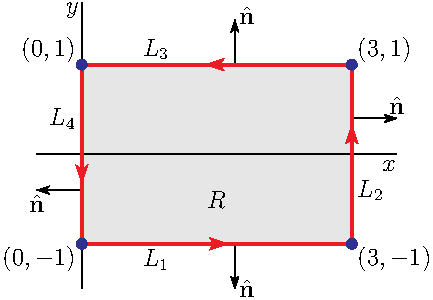
\includegraphics[scale=0.90]{OE16D_5.pdf}\
\end{center}

Its boundary consists of four line segments.
\begin{itemize}\itemsep1pt \parskip0pt \parsep0pt %\itemindent-15pt
\item[$\circ$]
$L_1$ from $(0,-1)$ to $(3,-1)$, with $\hn = -\hj$
\item[$\circ$]
$L_2$ from $(3,-1)$ to $(3,1)$, with $\hn = \hi$
\item[$\circ$]
$L_3$ from $(3,1)$ to $(0,1)$, with $\hn = \hj$
\item[$\circ$]
$L_4$ from $(0,1)$ to $(0,-1)$, with $\hn = -\hi$
\end{itemize}
So
\begin{align*}
\int_C \vF\cdot\hn\,\dee{s}
&= \int_{L_1} \vF\cdot(-\hj)\,\dee{s}
   +\int_{L_2} \vF\cdot \hi\,\dee{s}
   +\int_{L_3} \vF\cdot(\hj)\,\dee{s}
   +\int_{L_4} \vF\cdot(-\hi)\,\dee{s} \\
&= \int_0^3  -\overbrace{(-1)}^{y}e^x\,\dee{x}
   +\int_{-1}^1  \overbrace{(3)}^{x}y^2\,\dee{y}
   +\int^0_3  \overbrace{(1)}^{y}e^x\,\overbrace{(-\dee{x})}^{\dee{s}}
   +\int^{-1}_1  \overbrace{(0)}^{x}y^2\,\overbrace{(-\dee{y})}^{\dee{s}} \\
&=\big[e^3-1\big]+\big[1^3-(-1)^3\big] + \big[e^3-1\big]+0 \\
&=2e^3
\end{align*}
The trickiest part of this computation is getting $\dee{s}$ correct on
$L_3$ and $L_4$ (remembering that $\dee{s}$ is the arc length traveled
and so is positive, while $\dee{x}<0$ on $L_3$ and $\dee{y}<0$ on $L_4$).
To make a more detailed computation of $\int_{L_3} \vF\cdot(\hj)\,\dee{s}$,
parametrize $L_3$ by
\begin{equation*}
\vr(t) = (3,1) + t\big\{(0,1)-(3,1)\big\}
       = \big(3-3t,1\big)\qquad
0\le t\le 1
\end{equation*}
so that $\vr(0) = (3,1)$ is the initial point of $L_3$ and
$\vr(1) = (0,1)$ is the final point of $L_3$. Then
\begin{equation*}
\vr'(t) = (-3,0)\qquad
\diff{s}{t}(t) = |\vr'(t)| = 3
\end{equation*}
and
\begin{align*}
\int_{L_3} \vF\cdot \hj\,\dee{s}
=\int_0^1 \vF\big(\vr(t)\big)\cdot \hj\,\diff{s}{t}(t)\,\dee{t}
=\int_0^1\overbrace{e^{3-3t}}^{y(t)e^{x(t)}}\,
\overbrace{3}^{\diff{s}{t}(t)}\,\dee{t}
=-e^{3-3t}\Big|_0^1
=e^3-1
\end{align*}
\end{solution}


%%%%%%%%%%%%%%%%%%%%%%%%%%%%%%%
\begin{question}[M317 1998D] %1
	Let $\cC$ be the curve given by 
	$$
	\vr(t)=t\cos t\,\hi+t\sin t\,\hj+t^2\,\hk,\qquad 0\le t\le \pi
	$$
	\begin{enumerate}[(a)]
		\item
		Find the unit tangent $\hT$ to $\cC$ at the point $(-\pi,0,\pi^2)$.
		\item
		Calculate the line integral
		$$
		\int_\cC \sqrt{x^2+y^2}\ \dee{s}
		$$
		\item
		Find the equation of a smooth surface in $3$-space containing
		the curve $\cC$.
		\item
		Sketch the curve $\cC$.
	\end{enumerate}
\end{question}

\begin{hint} 
	(c) How is $x(t)^2+y(t)^2$ related to $z(t)$?
	
	(d) First, sketch $\big(x(t)\,,\,y(t)\big)$.
	
\end{hint}

\begin{answer} 
	(a) $\frac{1}{\sqrt{1+5\pi^2}}\big(-\hi-\pi\,\hj+2\pi\,\hk\big)$\qquad
	(b) $\frac{1}{15}\big[(1+5\pi^2)^{3/2}-1\big]$\qquad
	(c) $z=x^2+y^2$
	
	(d) 
	\begin{center}
		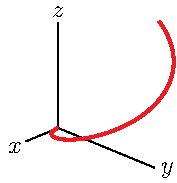
\includegraphics{OE98D_1.pdf}
	\end{center}
	
\end{answer}

\begin{solution} 
	(a) Since $\vr(t)=t\cos t\,\hi+t\sin t\,\hj+t^2\,\hk$
	\begin{align*}
		\vr'(t)&=\big(\cos t-t\sin t\big)\hi+\big(\sin t+t\cos t\big)\,\hj+2t\,\hk\\
		\diff{s}{t}
		&=|\vr'(t)|
		=\sqrt{\big(\cos t-t\sin t\big)^2+\big(\sin t+t\cos t\big)^2+(2t)^2}\\
		&=\sqrt{1+5t^2}\\
		\vr'(\pi)&=-\hi-\pi\,\hj+2\pi\,\hk\\
		\hat\vT(\pi)&=\frac{\vr'(t)}{|\vr'(t)|}
		=\frac{1}{\sqrt{1+5\pi^2}}\big(-\hi-\pi\,\hj+2\pi\,\hk\big)
	\end{align*}
	
	(b)
	\begin{align*}
		\int_\cC \sqrt{x^2+y^2}\ \dee{s}
		&=\int_0^\pi \sqrt{x^2(t)+y^2(t)}\ \diff{s}{t}\ \dee{t}
		=\int_0^\pi t\ \sqrt{1+5t^2}\ \dee{t}
		=\left[\frac{1}{15}(1+5t^2)^{3/2}\right]_0^\pi \\
		&=\frac{1}{15}\big[(1+5\pi^2)^{3/2}-1\big]
	\end{align*}
	
	(c) For every $t$, the coordinates $x(t)=t\cos t$, $y(t)=t\sin t$, 
	$z(t)=t^2$ obey $x(t)^2+y(t)^2= t^2 = z(t)$ and so the curve lies on
	$z=x^2+y^2$.
	
	(d) First concentrate on $\big(x(t)\,,\,y(t)\big)$. As $t$ runs from $0$
	to $\pi$, the curve $\big(r\cos t\,,\,r\sin t\big)$ sweeps out 
	half of a circle of radius $r$. Our  $\big(x(t)\,,\,y(t)\big)$
	does something similar, but the radius $r=t$ increases from $0$
	to $\pi$. Thus our $\big(x(t)\,,\,y(t)\big)$
	sweeps out the beginning of a spiral. At the same time $z(t)$
	increases from $0$ to $\pi^2$. So the curve $\cC$ looks like
	
	\begin{center}
		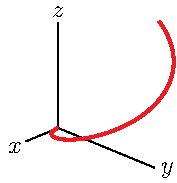
\includegraphics{OE98D_1.pdf}
	\end{center}
	
\end{solution}

%%%%%%%%%%%%%%%%%%%
\begin{question}
A wire traces out a path $C$  described by the curve $(t+\frac12t^2~,~t-\frac12t^2~,~\frac{4}{3}\,t^{3/2})$, $0 \leq t \leq 4$. Its density at the point $(x,y,z)$ is $\rho(x,y,z)={\left( \frac{x+y}{2}\right)}$. Find its centre of mass.
\end{question}
\begin{hint}
	Remember $\bar x = \dfrac{\int_C x\rho\,\dee{s}}{\int_C \rho\,\dee{s}}$, etc. The integrals you evaluate should all be straightforward applications of the power rule.
\end{hint}
\begin{answer}
	$\left( \frac{412}{55},-\frac{92}{55},\frac{4736}{693}\right)$
\end{answer}
\begin{solution}
We use the centre of mass formulae $\bar x = \dfrac{\int_C x\rho\,\dee{s}}{\int_C \rho\,\dee{s}}$, etc. To make the working clearer, we'll break these calculations into several steps.
\begin{align*}
x(t)&= t+ \frac12 t^2 & x'(t)&=1+t\\
y(t)&= t- \frac12 t^2 & y'(t)&=1-t\\
z(t)&=\frac43 t^{3/2} & z'(t)&=2\sqrt{t}
\end{align*}
\begin{align*}
\color{blue}\sqrt{x'(t)^2+y'(t)^2+z'(t)^2}&=\sqrt{1+2t+t^2+1-2t+t^2+4t}=\sqrt{2(t^2+2t+1)}=\textcolor{blue}{\sqrt{2}(t+1)}\\
\color{red}\rho(x(t),y(t),z(t))&= \frac{x(t)+y(t)}{2}={\frac{(t+t^2/2 )+( t -  t^2/2)}{2}}=\textcolor{red}{t}
\end{align*}
\begin{align*}
\int_C \textcolor{red}\rho \,\dee{s}&=\int_0^4 \textcolor{red}{t}\,\textcolor{blue}{\sqrt{2}(t+1)}\,\dee{t}
=\frac{2^3\cdot 11\sqrt{2}}{3}\displaybreak[0]\\
\int_C x \textcolor{red}\rho \,\dee{s}&=\int_0^4 \left(t+\frac12t^2\right) \textcolor{red}{t}\,\textcolor{blue}{\sqrt{2}(t+1)}\,\dee{t}
=\sqrt{2}\int_0^{2^2} \left(\frac{t^4}{2}+\frac{3}{2}t^3
                                 +t^2\right)\ \dee{t}\\
            &=\sqrt{2}\left(\frac{2^9}{5} +3(2^5)+\frac{2^6}{3}\right)
=\frac{2^5\cdot103\sqrt 2}{15}\displaybreak[0]\\
\int_C y \textcolor{red}\rho \,\dee{s}&=\int_0^4 \left(t-\frac12t^2\right)\textcolor{red}{t}\, \textcolor{blue}{\sqrt{2}(t+1)}\,\dee{t}=\sqrt2\int_0^{2^2}\left(-\frac{t^4}{2}+\frac{t^3}{2}+t^2 \right)\dee{t}\\
&=\sqrt{2}\left(-\frac{2^9}{5}+{2^5}+\frac{2^6}{3} \right) 
=-\frac{2^5\cdot 23\sqrt 2}{15}\displaybreak[0]\\
\int_C z \textcolor{red} \rho\, \dee{s}&=\int_0^4 \left(\frac{4}{3}t^{3/2}\right) \textcolor{red}{t}\, \textcolor{blue}{\sqrt{2}(t+1)}\,\dee{t}=\frac{4\sqrt2}{3}\int_0^{2^2} 
\left( t^{7/2}+t^{5/2}\right)\dee{t}\\
&=\frac{4\sqrt2}{3}\left( \frac{2^{10}}{9}+\frac{2^8}{7}\right)=\frac{2^{10}\cdot37\sqrt{2}}{7\cdot 3^3}
\displaybreak[0]\\
\overline{x}&=\frac{\int x \rho\,\dee{s}}{\int \rho\,\dee{s}}=\frac{\frac{2^5\cdot103\sqrt 2}{15}}{\frac{2^3\cdot 11\sqrt{2}}{3}}=\frac{412}{55}\approx 7.5\\
\overline{y}&=\frac{\int y \rho\,\dee{s}}{\int \rho\,\dee{s}}=\frac{-\frac{2^5\cdot 23\sqrt 2}{15}}{\frac{2^3\cdot 11\sqrt{2}}{3}}=-\frac{92}{55}\approx-1.7\\
\overline{z}&=\frac{\int z \rho\,\dee{s}}{\int \rho\,\dee{s}}=\frac{\frac{2^{10}\cdot37\sqrt{2}}{7\cdot 3^3}}{\frac{2^3\cdot 11\sqrt{2}}{3}}=\frac{4736}{693}\approx 6.8
\end{align*}

After these long calculations, it's nice to do a sanity check. Using $0 \le t \le 4$, we see our wire takes up space in the following intervals: $0 \le x \le 12$, $-4 \le y \le 1/2$, and $0 \le z \le 32/3$. The coordinates of our centre of mass all fall in these intervals, which doesn't guarantee our answer is correct, but it is a nice sign. If, say $\overline x$ had been negative, or $\overline z$ were greater than 11, we would have known there was something wrong.
\end{solution}
%%%%%%%%%%%%%%%%%%%
